\chapter{Architectures}\label{Architectures}

Finding a suitable architecture is a vital step in creating a well-performant deep learning model. By leveraging different techniques, we balance introduction of inductive biases and possibility for complexity, which hopefully can help us end up with a generalizing model.

We train a model suitable at predicting the largest common vocabulary in \gls{ADT}, namely the 5-class vocabulary consisting of \acrfull{KD}, \acrfull{SD}, \acrfull{TT}, \acrfull{HH}, \acrfull{CC+RC}~\cite{zehren2024analyzingreducingsynthetictorealtransfer}.

\section{Recurrent Neural Network}

The \gls{RNN} is a standard architecture when it comes prediction on sequence data. It has been tried and tested, showing promising results for audio tasks.

The fundamental building block for \glspl{RNN} is the \textit{recurrent unit}. It iterates the whole input sequence, storing information from previous timesteps in a form of memory, through maintenance of a \textit{hidden state}. This can be extended to gaining information about future timesteps by using \textit{bidirectional} versions. In this way, prediction on current timesteps are affected by the information from surrounding timesteps. This is relevant in tasks such as \gls{ADT} as auditory information usually spreads over several timesteps, e.g. the timbre of an instrument event lingering after onset.

\begin{figure}[H]
    \centering
    \usetikzlibrary{positioning, chains, shapes.geometric, fit, shapes, arrows.meta, calc, backgrounds}

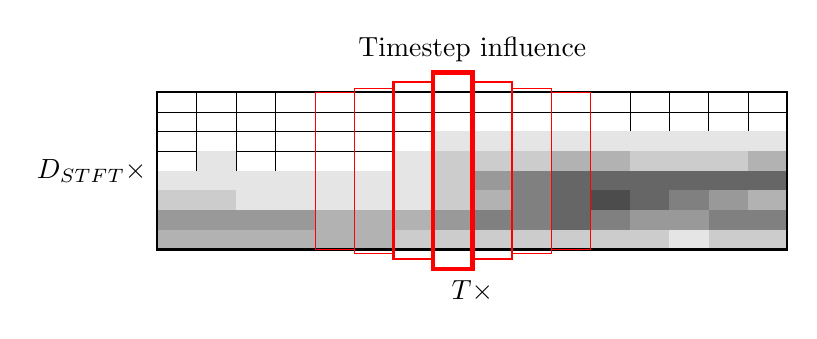
\begin{tikzpicture}[
    very thick,
    arrow/.style={
        -latex,
        very thick,
        rounded corners=0.2cm
    },
    ]

% ------ Grid ------

\draw[transform canvas={xscale=2}, step=0.25cm, ultra thin] (-2, 1) grid (2, 3);
\node[anchor=south] at (0, 3.25) {Timestep influence};
\node[anchor=east] at (-4, 2) {$D_\text{STFT}\times$};
\node[anchor=north] at (0, 0.75) {$T\times$};

% ------ Values ------

\fill[black!30] (-4.0, 1.0) rectangle (-3.5, 1.25);
\fill[black!30] (-3.5, 1.0) rectangle (-3.0, 1.25);
\fill[black!30] (-3.0, 1.0) rectangle (-2.5, 1.25);
\fill[black!30] (-2.5, 1.0) rectangle (-2.0, 1.25);
\fill[black!30] (-2.0, 1.0) rectangle (-1.5, 1.25);
\fill[black!30] (-1.5, 1.0) rectangle (-1.0, 1.25);
\fill[black!20] (-1.0, 1.0) rectangle (-0.5, 1.25);
\fill[black!20] (-0.5, 1.0) rectangle (0.0, 1.25);
\fill[black!20] (0.0, 1.0) rectangle (0.5, 1.25);
\fill[black!20] (0.5, 1.0) rectangle (1.0, 1.25);
\fill[black!20] (1.0, 1.0) rectangle (1.5, 1.25);
\fill[black!20] (1.5, 1.0) rectangle (2.0, 1.25);
\fill[black!20] (2.0, 1.0) rectangle (2.5, 1.25);
\fill[black!10] (2.5, 1.0) rectangle (3.0, 1.25);
\fill[black!20] (3.0, 1.0) rectangle (3.5, 1.25);
\fill[black!20] (3.5, 1.0) rectangle (4.0, 1.25);
\fill[black!40] (-4.0, 1.25) rectangle (-3.5, 1.5);
\fill[black!40] (-3.5, 1.25) rectangle (-3.0, 1.5);
\fill[black!40] (-3.0, 1.25) rectangle (-2.5, 1.5);
\fill[black!40] (-2.5, 1.25) rectangle (-2.0, 1.5);
\fill[black!30] (-2.0, 1.25) rectangle (-1.5, 1.5);
\fill[black!30] (-1.5, 1.25) rectangle (-1.0, 1.5);
\fill[black!30] (-1.0, 1.25) rectangle (-0.5, 1.5);
\fill[black!40] (-0.5, 1.25) rectangle (0.0, 1.5);
\fill[black!50] (0.0, 1.25) rectangle (0.5, 1.5);
\fill[black!50] (0.5, 1.25) rectangle (1.0, 1.5);
\fill[black!60] (1.0, 1.25) rectangle (1.5, 1.5);
\fill[black!50] (1.5, 1.25) rectangle (2.0, 1.5);
\fill[black!40] (2.0, 1.25) rectangle (2.5, 1.5);
\fill[black!40] (2.5, 1.25) rectangle (3.0, 1.5);
\fill[black!50] (3.0, 1.25) rectangle (3.5, 1.5);
\fill[black!50] (3.5, 1.25) rectangle (4.0, 1.5);
\fill[black!20] (-4.0, 1.5) rectangle (-3.5, 1.75);
\fill[black!20] (-3.5, 1.5) rectangle (-3.0, 1.75);
\fill[black!10] (-3.0, 1.5) rectangle (-2.5, 1.75);
\fill[black!10] (-2.5, 1.5) rectangle (-2.0, 1.75);
\fill[black!10] (-2.0, 1.5) rectangle (-1.5, 1.75);
\fill[black!10] (-1.5, 1.5) rectangle (-1.0, 1.75);
\fill[black!10] (-1.0, 1.5) rectangle (-0.5, 1.75);
\fill[black!20] (-0.5, 1.5) rectangle (0.0, 1.75);
\fill[black!30] (0.0, 1.5) rectangle (0.5, 1.75);
\fill[black!50] (0.5, 1.5) rectangle (1.0, 1.75);
\fill[black!60] (1.0, 1.5) rectangle (1.5, 1.75);
\fill[black!70] (1.5, 1.5) rectangle (2.0, 1.75);
\fill[black!60] (2.0, 1.5) rectangle (2.5, 1.75);
\fill[black!50] (2.5, 1.5) rectangle (3.0, 1.75);
\fill[black!40] (3.0, 1.5) rectangle (3.5, 1.75);
\fill[black!30] (3.5, 1.5) rectangle (4.0, 1.75);
\fill[black!10] (-4.0, 1.75) rectangle (-3.5, 2.0);
\fill[black!10] (-3.5, 1.75) rectangle (-3.0, 2.0);
\fill[black!10] (-3.0, 1.75) rectangle (-2.5, 2.0);
\fill[black!10] (-2.5, 1.75) rectangle (-2.0, 2.0);
\fill[black!10] (-2.0, 1.75) rectangle (-1.5, 2.0);
\fill[black!10] (-1.5, 1.75) rectangle (-1.0, 2.0);
\fill[black!10] (-1.0, 1.75) rectangle (-0.5, 2.0);
\fill[black!20] (-0.5, 1.75) rectangle (0.0, 2.0);
\fill[black!40] (0.0, 1.75) rectangle (0.5, 2.0);
\fill[black!50] (0.5, 1.75) rectangle (1.0, 2.0);
\fill[black!60] (1.0, 1.75) rectangle (1.5, 2.0);
\fill[black!60] (1.5, 1.75) rectangle (2.0, 2.0);
\fill[black!60] (2.0, 1.75) rectangle (2.5, 2.0);
\fill[black!60] (2.5, 1.75) rectangle (3.0, 2.0);
\fill[black!60] (3.0, 1.75) rectangle (3.5, 2.0);
\fill[black!60] (3.5, 1.75) rectangle (4.0, 2.0);
\fill[black!10] (-3.5, 2.0) rectangle (-3.0, 2.25);
\fill[black!10] (-1.0, 2.0) rectangle (-0.5, 2.25);
\fill[black!20] (-0.5, 2.0) rectangle (0.0, 2.25);
\fill[black!20] (0.0, 2.0) rectangle (0.5, 2.25);
\fill[black!20] (0.5, 2.0) rectangle (1.0, 2.25);
\fill[black!30] (1.0, 2.0) rectangle (1.5, 2.25);
\fill[black!30] (1.5, 2.0) rectangle (2.0, 2.25);
\fill[black!20] (2.0, 2.0) rectangle (2.5, 2.25);
\fill[black!20] (2.5, 2.0) rectangle (3.0, 2.25);
\fill[black!20] (3.0, 2.0) rectangle (3.5, 2.25);
\fill[black!30] (3.5, 2.0) rectangle (4.0, 2.25);
\fill[black!10] (-0.5, 2.25) rectangle (0.0, 2.5);
\fill[black!10] (0.0, 2.25) rectangle (0.5, 2.5);
\fill[black!10] (0.5, 2.25) rectangle (1.0, 2.5);
\fill[black!10] (1.0, 2.25) rectangle (1.5, 2.5);
\fill[black!10] (1.5, 2.25) rectangle (2.0, 2.5);
\fill[black!10] (2.0, 2.25) rectangle (2.5, 2.5);
\fill[black!10] (2.5, 2.25) rectangle (3.0, 2.5);
\fill[black!10] (3.0, 2.25) rectangle (3.5, 2.5);
\fill[black!10] (3.5, 2.25) rectangle (4.0, 2.5);

% ------ Outline ------
\draw[thick] (-4, 1) -- (4, 1) -- (4, 3) -- (-4, 3) -- cycle;

% ------ Influence ------

\draw[ultra thick, color=red] (-0.5, 0.75) -- (0, 0.75) -- (0, 3.25) -- (-0.5, 3.25) -- cycle;

\draw[thick, color=red] (-1, 0.875) -- (-0.5, 0.875) -- (-0.5, 3.125) -- (-1, 3.125) -- cycle;
\draw[thick, color=red] (0, 0.875) -- (0.5, 0.875) -- (0.5, 3.125) -- (0, 3.125) -- cycle;

\draw[thin, color=red] (-1.5, 0.95) -- (-1, 0.95) -- (-1, 3.05) -- (-1.5, 3.05) -- cycle;
\draw[thin, color=red] (0.5, 0.95) -- (1, 0.95) -- (1, 3.05) -- (0.5, 3.05) -- cycle;

\draw[ultra thin, color=red] (-2, 1) -- (-1.5, 1) -- (-1.5, 3) -- (-2, 3) -- cycle;
\draw[ultra thin, color=red] (1, 1) -- (1.5, 1) -- (1.5, 3) -- (1, 3) -- cycle;

\end{tikzpicture}
    \caption{An example of how bidirectional \glspl{RNN} allow for adjacent timesteps to influence the prediction of the current timestep. The background is a spectrogram, and the red boxes represent influence in the middle timeframe. The height of the box help visualize influence strength.}
    \label{RNNInfluenceFigure}
\end{figure}

However, traditional \glspl{RNN} suffer from the \textit{vanishing gradient problem} due to a timestep's influence diminishing with distance, making \textit{long range dependencies} harder to learn. Different architectures have been developed to try to overcome these issues, such as the \gls{GRU} by Cho et al.~\cite{DBLP:conf/emnlp/ChoMGBBSB14}, and \gls{LSTM} by Hochreiter and Schmidhuber~\cite{10.1162/neco.1997.9.8.1735}.

It has been shown that \glspl{GRU} and \glspl{LSTM} are capable of learning \gls{ADT} related tasks, and is therefore in interest to comparatively measure how their efficiency stands in regards to other architectures~\cite{Southall2016AutomaticDT, vogl2016recurrent, Vogl2017DrumTV, signals4040042}.

\subsection{Implementation}

Our \gls{RNN} architecture consists of several bidirectional recurrent units, ending in a framewise linear layer. For the \gls{BiRU}, we train either a \gls{GRU} or an \gls{LSTM} model as hyperparameters, in addition to search over number of layers $L$ and hidden size $H$, selecting the one with best performance. At last, we have a linear layer, outputting onset probabilities for each of the drums per timeframe.

\begin{figure}[H]
    \centering
    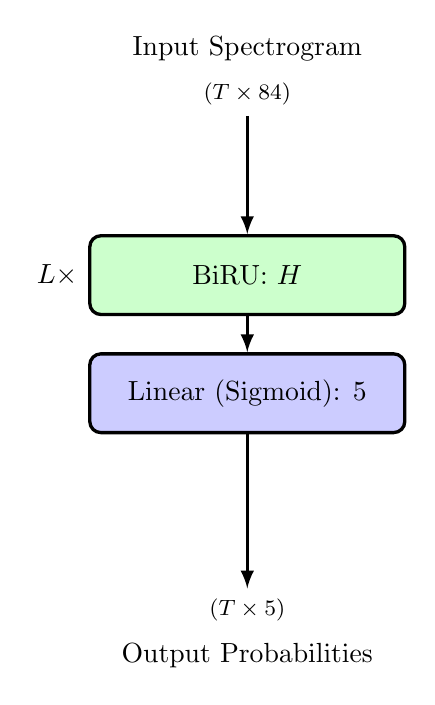
\begin{tikzpicture}[
    very thick,
    arrow/.style={
        -latex,
        very thick,
        rounded corners=0.2cm
    },
    ]

\node[anchor=south, label=above:{Input Spectrogram}] at (0, 0){\footnotesize{($T \times 84$)}};

\draw[arrow] (0, 0) -- (0, -1.5) node[rectangle, 
rounded corners, 
draw, 
anchor=north, 
label=west:$L\times$,
fill=green!20,
minimum height=1cm,
minimum width=4cm
] (a) {\acrshort{BiRU}: $H$};

\draw[arrow] (a) -- (0, -3) node[rectangle, 
rounded corners, 
draw, 
anchor=north, 
fill=blue!20,
minimum height=1cm,
minimum width=4cm
] (b) {Linear (Sigmoid): $5$};

\draw[arrow] (b) -- (0, -6);

\node[anchor=north, label=below:{Output Probabilities}] at (0, -6){\footnotesize{($T \times 5$)}};

\end{tikzpicture}
    \caption{RNN architecture structure.}
    \label{RNNFigure}
\end{figure}

\begin{table}[H]
    \centering
    \begin{tabular}{lr|c}
        \multicolumn{2}{c|}{Hyperparameter} & Values       \\
        \hline
        $L$ & Number of layers      & \{2, 3, 4, 5, 6\} \\
        $H$ & Hidden size      & \{72, 144, 288, 576\} \\
        \gls{BiRU} & \acrlong{BiRU} & \{\gls{GRU}, \gls{LSTM}\}\\
    \end{tabular}
    \caption{The different hyperparameters and their respective values tuned to train the Recurrent Neural Network.}
    \label{RNNHyperparams}
\end{table}

\section{Convolutional Neural Network}

We've mentioned that spectrograms can be treated as images. Therefore it would make sense to try an image focused approach, by utilizing \textit{convolutions}. By applying convolutional layers, each timestep gets access to information around itself, a \textit{context}. These convolutional layers make up the primary building blocks for the \gls{CNN}.

\begin{figure}[H]
    \centering
    \begin{tikzpicture}[
    very thick,
    arrow/.style={
        -latex,
        very thick,
        rounded corners=0.2cm
    },
    ]

% ------ Grid ------

\draw[transform canvas={xscale=2}, step=0.25cm, ultra thin] (-2, 1) grid (2, 3);
\node[anchor=south] at (0, 3.25) {Contextual influence};
\node[anchor=east] at (-4, 2) {$D_\text{STFT}\times$};
\node[anchor=north] at (0, 0.75) {$T\times$};

% ------ Values ------

\fill[black!30] (-4.0, 1.0) rectangle (-3.5, 1.25);
\fill[black!30] (-3.5, 1.0) rectangle (-3.0, 1.25);
\fill[black!30] (-3.0, 1.0) rectangle (-2.5, 1.25);
\fill[black!30] (-2.5, 1.0) rectangle (-2.0, 1.25);
\fill[black!30] (-2.0, 1.0) rectangle (-1.5, 1.25);
\fill[black!30] (-1.5, 1.0) rectangle (-1.0, 1.25);
\fill[black!20] (-1.0, 1.0) rectangle (-0.5, 1.25);
\fill[black!20] (-0.5, 1.0) rectangle (0.0, 1.25);
\fill[black!20] (0.0, 1.0) rectangle (0.5, 1.25);
\fill[black!20] (0.5, 1.0) rectangle (1.0, 1.25);
\fill[black!20] (1.0, 1.0) rectangle (1.5, 1.25);
\fill[black!20] (1.5, 1.0) rectangle (2.0, 1.25);
\fill[black!20] (2.0, 1.0) rectangle (2.5, 1.25);
\fill[black!10] (2.5, 1.0) rectangle (3.0, 1.25);
\fill[black!20] (3.0, 1.0) rectangle (3.5, 1.25);
\fill[black!20] (3.5, 1.0) rectangle (4.0, 1.25);
\fill[black!40] (-4.0, 1.25) rectangle (-3.5, 1.5);
\fill[black!40] (-3.5, 1.25) rectangle (-3.0, 1.5);
\fill[black!40] (-3.0, 1.25) rectangle (-2.5, 1.5);
\fill[black!40] (-2.5, 1.25) rectangle (-2.0, 1.5);
\fill[black!30] (-2.0, 1.25) rectangle (-1.5, 1.5);
\fill[black!30] (-1.5, 1.25) rectangle (-1.0, 1.5);
\fill[black!30] (-1.0, 1.25) rectangle (-0.5, 1.5);
\fill[black!40] (-0.5, 1.25) rectangle (0.0, 1.5);
\fill[black!50] (0.0, 1.25) rectangle (0.5, 1.5);
\fill[black!50] (0.5, 1.25) rectangle (1.0, 1.5);
\fill[black!60] (1.0, 1.25) rectangle (1.5, 1.5);
\fill[black!50] (1.5, 1.25) rectangle (2.0, 1.5);
\fill[black!40] (2.0, 1.25) rectangle (2.5, 1.5);
\fill[black!40] (2.5, 1.25) rectangle (3.0, 1.5);
\fill[black!50] (3.0, 1.25) rectangle (3.5, 1.5);
\fill[black!50] (3.5, 1.25) rectangle (4.0, 1.5);
\fill[black!20] (-4.0, 1.5) rectangle (-3.5, 1.75);
\fill[black!20] (-3.5, 1.5) rectangle (-3.0, 1.75);
\fill[black!10] (-3.0, 1.5) rectangle (-2.5, 1.75);
\fill[black!10] (-2.5, 1.5) rectangle (-2.0, 1.75);
\fill[black!10] (-2.0, 1.5) rectangle (-1.5, 1.75);
\fill[black!10] (-1.5, 1.5) rectangle (-1.0, 1.75);
\fill[black!10] (-1.0, 1.5) rectangle (-0.5, 1.75);
\fill[black!20] (-0.5, 1.5) rectangle (0.0, 1.75);
\fill[black!30] (0.0, 1.5) rectangle (0.5, 1.75);
\fill[black!50] (0.5, 1.5) rectangle (1.0, 1.75);
\fill[black!60] (1.0, 1.5) rectangle (1.5, 1.75);
\fill[black!70] (1.5, 1.5) rectangle (2.0, 1.75);
\fill[black!60] (2.0, 1.5) rectangle (2.5, 1.75);
\fill[black!50] (2.5, 1.5) rectangle (3.0, 1.75);
\fill[black!40] (3.0, 1.5) rectangle (3.5, 1.75);
\fill[black!30] (3.5, 1.5) rectangle (4.0, 1.75);
\fill[black!10] (-4.0, 1.75) rectangle (-3.5, 2.0);
\fill[black!10] (-3.5, 1.75) rectangle (-3.0, 2.0);
\fill[black!10] (-3.0, 1.75) rectangle (-2.5, 2.0);
\fill[black!10] (-2.5, 1.75) rectangle (-2.0, 2.0);
\fill[black!10] (-2.0, 1.75) rectangle (-1.5, 2.0);
\fill[black!10] (-1.5, 1.75) rectangle (-1.0, 2.0);
\fill[black!10] (-1.0, 1.75) rectangle (-0.5, 2.0);
\fill[black!20] (-0.5, 1.75) rectangle (0.0, 2.0);
\fill[black!40] (0.0, 1.75) rectangle (0.5, 2.0);
\fill[black!50] (0.5, 1.75) rectangle (1.0, 2.0);
\fill[black!60] (1.0, 1.75) rectangle (1.5, 2.0);
\fill[black!60] (1.5, 1.75) rectangle (2.0, 2.0);
\fill[black!60] (2.0, 1.75) rectangle (2.5, 2.0);
\fill[black!60] (2.5, 1.75) rectangle (3.0, 2.0);
\fill[black!60] (3.0, 1.75) rectangle (3.5, 2.0);
\fill[black!60] (3.5, 1.75) rectangle (4.0, 2.0);
\fill[black!10] (-3.5, 2.0) rectangle (-3.0, 2.25);
\fill[black!10] (-1.0, 2.0) rectangle (-0.5, 2.25);
\fill[black!20] (-0.5, 2.0) rectangle (0.0, 2.25);
\fill[black!20] (0.0, 2.0) rectangle (0.5, 2.25);
\fill[black!20] (0.5, 2.0) rectangle (1.0, 2.25);
\fill[black!30] (1.0, 2.0) rectangle (1.5, 2.25);
\fill[black!30] (1.5, 2.0) rectangle (2.0, 2.25);
\fill[black!20] (2.0, 2.0) rectangle (2.5, 2.25);
\fill[black!20] (2.5, 2.0) rectangle (3.0, 2.25);
\fill[black!20] (3.0, 2.0) rectangle (3.5, 2.25);
\fill[black!30] (3.5, 2.0) rectangle (4.0, 2.25);
\fill[black!10] (-0.5, 2.25) rectangle (0.0, 2.5);
\fill[black!10] (0.0, 2.25) rectangle (0.5, 2.5);
\fill[black!10] (0.5, 2.25) rectangle (1.0, 2.5);
\fill[black!10] (1.0, 2.25) rectangle (1.5, 2.5);
\fill[black!10] (1.5, 2.25) rectangle (2.0, 2.5);
\fill[black!10] (2.0, 2.25) rectangle (2.5, 2.5);
\fill[black!10] (2.5, 2.25) rectangle (3.0, 2.5);
\fill[black!10] (3.0, 2.25) rectangle (3.5, 2.5);
\fill[black!10] (3.5, 2.25) rectangle (4.0, 2.5);

% ------ Outline ------
\draw[thick] (-4, 1) -- (4, 1) -- (4, 3) -- (-4, 3) -- cycle;

% ------ Influence ------

\draw[ultra thick, color=red, pattern=north east lines, pattern color=red] (-0.5, 1) -- (0, 1) -- (0, 3) -- (-0.5, 3) -- cycle;

\draw[thick, color=red] (-1, 1) -- (0.5, 1) -- (0.5, 3.) -- (-1, 3) -- cycle;


\end{tikzpicture}
    \caption{An example of how \glspl{CNN} allow for a fixed context of influence from neighbouring timesteps when predicting each timestep. The background is a spectrogram, and the red boxes represent influence in the middle timeframe, being described by the red shaded region.}
    \label{CNNInfluenceFigure}
\end{figure}

\glspl{CNN} have been shown to give reasonable performance within \gls{ADT}. This could be due to contextual information being important for identifying instrument onsets, and making learning easier for our models~\cite{Vogl2017DrumTV}.

\subsection{Implementation}

Our \gls{CNN} architecure consists of $I$ initial convolutional blocks. Inside this block, convolutional layers have an increasing number of kernels $C = \{32, 64, 96\}$, intuitively leading to an increase in complexity along with depth. Note that this is not a hyperparameter, but just denotes that we increase the amount of kernels the deeper into the convolutional block we go. Then we have a varying amount of fully connected layers $L$, projecting into a latent space sized $H$. Both the convolutional and fully connected layers are followed by a \gls{ReLU} activation function. Lastly, an output layer computed each instrument's onset probabilities.

\begin{figure}[H]
    \centering
    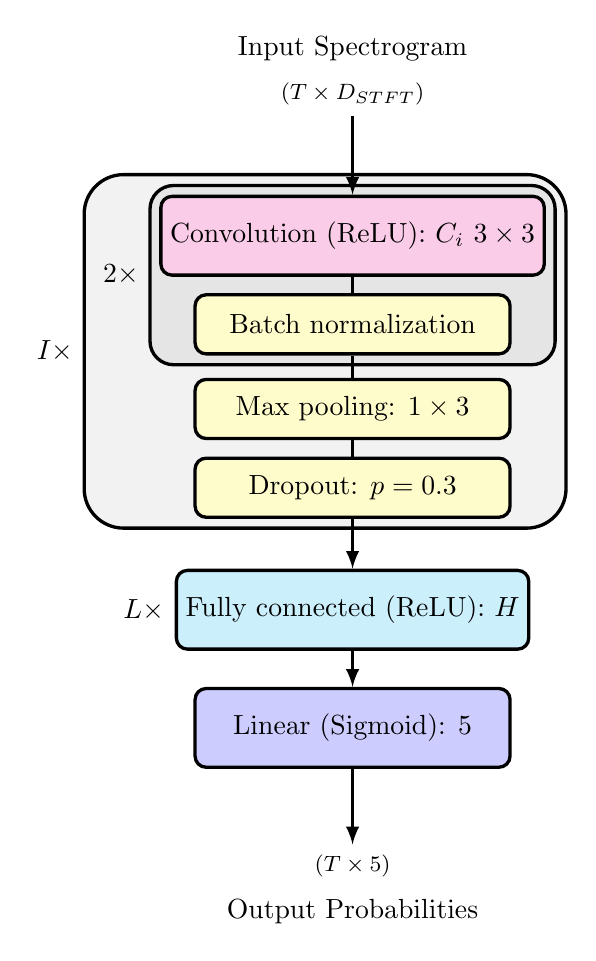
\begin{tikzpicture}[
    very thick,
    arrow/.style={
        -latex,
        very thick,
        rounded corners=0.2cm
    },
    ]

\node[anchor=south, label=above:{Input Spectrogram}] at (0, -0.5){\footnotesize{($T \times D_\text{STFT}$)}};

\draw[arrow] (0, -0.5) -- (0, -1.5) node [rectangle,
rounded corners,
draw,
anchor=north,
fill=magenta!20,
minimum height=1cm,
minimum width=4cm
] (a) {Convolution (ReLU): $C_i$  $3 \times 3$};

\draw (a) -- (0, -2.75) node[rectangle,
rounded corners,
draw,
anchor=north,
fill=yellow!20,
minimum height=0.75cm,
minimum width=4cm
] (b) {Batch normalization};

\draw (b) -- (0, -3.825) node[rectangle,
rounded corners,
draw,
anchor=north,
fill=yellow!20,
minimum height=0.75cm,
minimum width=4cm
] (c) {Max pooling: $1 \times 3$};

\draw (c) -- (0, -4.825) node[rectangle,
rounded corners,
draw,
anchor=north,
fill=yellow!20,
minimum height=0.75cm,
minimum width=4cm
] (d) {Dropout: $p = 0.3$};

\begin{scope}[on background layer]
    \node[rectangle,
    fill=gray!20,
    rounded corners=3mm,
    label={[name=ablabel]west:$2\times$},
    draw,
    very thick,
    fit=(a) (b)] (ab) {};
    \node[rectangle,
    fill=gray!10,
    rounded corners=5mm,
    label=west:$I\times$,
    draw,
    very thick,
    fit= (ab) (ablabel) (d)] {};
    \node[rectangle,
    fill=gray!20,
    rounded corners=3mm,
    label={[name=ablabel]west:$2\times$},
    draw,
    very thick,
    fit=(a) (b)] (ab) {};
\end{scope}


\draw[arrow] (d) -- (0, -6.25) node[rectangle, 
rounded corners, 
draw, 
anchor=north, 
label=west:$L\times$,
fill=cyan!20,
minimum height=1cm,
minimum width=4cm
] (g) {Fully connected (ReLU): $H$};

\draw[arrow] (g) -- (0, -7.75) node[rectangle, 
rounded corners, 
draw, 
anchor=north, 
fill=blue!20,
minimum height=1cm,
minimum width=4cm
] (h) {Linear (Sigmoid): $5$};

\draw[arrow] (h) -- (0, -9.75);

\node[anchor=north, label=below:{Output Probabilities}] at (0, -9.75){\footnotesize{($T \times 5$)}};

\end{tikzpicture}
    \caption{CNN architecture structure.}
    \label{CNNFigure}
\end{figure}

\begin{table}[H]
    \centering
    \begin{tabular}{lr|c}
        \multicolumn{2}{c|}{Hyperparameter} & Values       \\
        \hline
        $I$ & Number of convolutions & \{1, 2, 3\}\\
        $L$ & Number of layers      & \{2, 3, 4\} \\
        $H$ & Hidden size      & \{72, 144, 288, 576\} \\
    \end{tabular}
    \caption{The different hyperparameters and their respective values tuned to train the Convolutional Neural Network.}
    \label{CNNHyperparams}
\end{table}

\section[Convolutional RNN]{Convolutional Recurrent Neural Network}

The previous features, recurrent layers and convolutions, are not mutually exclusive. Theoretically they can harmonize together, complementing eachother for easier learning. This results in the \gls{CRNN} architecture.

Intuitively, the \glspl{CNN} ability to process images like the spectrogram, together with the \glspl{RNN} ability to understand temporal sequence data should prove beneficial for \gls{ADT} tasks. And indeed, this combination of cross-timestep memory and contextual data representation has shown to be insightful~\cite{Vogl2017DrumTV, vogl2018multiinstrumentdrumtranscription, signals4040042}.

\subsection{Implementation}

We begin with a fixed-size convolutional block with $I = 2$, as used by several \gls{ADT} authors~\cite{Vogl2017DrumTV, signals4040042}. Following the \gls{CNN}, it has an increasing number of kernels $C = \{32, 64\}$ the deeper into the convolutions we go. We then, similar to the \gls{RNN}, have a \gls{BiRU} layer of either a \gls{GRU} or \gls{LSTM}, with number of layers $L \in \{2, 3, 4, 5\}$ and hidden size $H \in \{72, 144, 288\}$. Output probabilities are then computed through the final linear layer.

\begin{figure}[H]
    \centering
    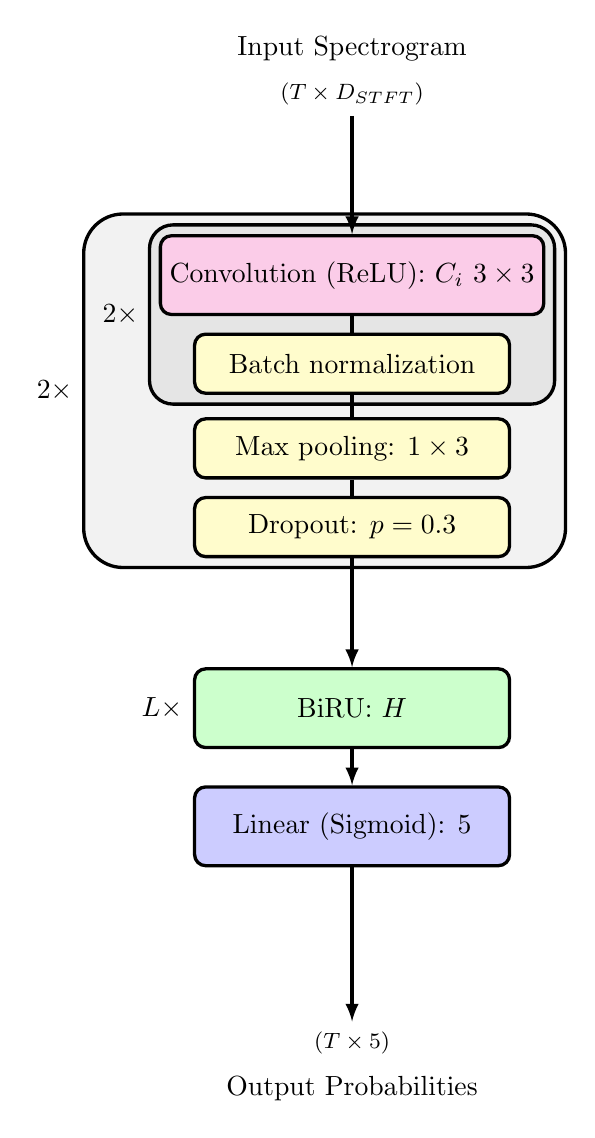
\begin{tikzpicture}[
    very thick,
    arrow/.style={
        -latex,
        very thick,
        rounded corners=0.2cm
    },
    ]

\node[anchor=south, label=above:{Input Spectrogram}] at (0, 0){\footnotesize{($T \times D_\text{STFT}$)}};

\draw[arrow] (0, 0) -- (0, -1.5) node [rectangle,
rounded corners,
draw,
anchor=north,
fill=magenta!20,
minimum height=1cm,
minimum width=4cm
] (a) {Convolution (ReLU): $C_i$  $3 \times 3$};

\draw (a) -- (0, -2.75) node[rectangle,
rounded corners,
draw,
anchor=north,
fill=yellow!20,
minimum height=0.75cm,
minimum width=4cm
] (b) {Batch normalization};

\draw (b) -- (0, -3.825) node[rectangle,
rounded corners,
draw,
anchor=north,
fill=yellow!20,
minimum height=0.75cm,
minimum width=4cm
] (c) {Max pooling: $1 \times 3$};

\draw (c) -- (0, -4.825) node[rectangle,
rounded corners,
draw,
anchor=north,
fill=yellow!20,
minimum height=0.75cm,
minimum width=4cm
] (d) {Dropout: $p = 0.3$};

\begin{scope}[on background layer]
    \node[rectangle,
    fill=gray!20,
    rounded corners=3mm,
    label={[name=ablabel]west:$2\times$},
    draw,
    very thick,
    fit=(a) (b)] (ab) {};
    \node[rectangle,
    fill=gray!10,
    rounded corners=5mm,
    label=west:$2\times$,
    draw,
    very thick,
    fit= (ab) (ablabel) (d)] {};
    \node[rectangle,
    fill=gray!20,
    rounded corners=3mm,
    label={[name=ablabel]west:$2\times$},
    draw,
    very thick,
    fit=(a) (b)] (ab) {};
\end{scope}

\draw[arrow] (d) -- (0, -7) node[rectangle, 
rounded corners, 
draw, 
anchor=north, 
label=west:$L\times$,
fill=green!20,
minimum height=1cm,
minimum width=4cm
] (g) {BiRU: $H$};

\draw[arrow] (g) -- (0, -8.5) node[rectangle, 
rounded corners, 
draw, 
anchor=north, 
fill=blue!20,
minimum height=1cm,
minimum width=4cm
] (h) {Linear (Sigmoid): $5$};

\draw[arrow] (h) -- (0, -11.5);

\node[anchor=north, label=below:{Output Probabilities}] at (0, -11.5){\footnotesize{($T \times 5$)}};

\end{tikzpicture}
    \caption{Convolutional RNN architecture structure.}
    \label{CRNNFigure}
\end{figure}

\begin{table}[H]
    \centering
    \begin{tabular}{lr|c}
        \multicolumn{2}{c|}{Hyperparameter} & Values       \\
        \hline
        $L$ & Number of layers      & \{2, 3, 4, 5\} \\
        $H$ & Hidden size      & \{72, 144, 288, 576\} \\
        \gls{BiRU} & \acrlong{BiRU} & \{\gls{GRU}, \gls{LSTM}\}\\
    \end{tabular}
    \caption{The different hyperparameters and their respective values tuned to train the Convolutional Recurrent Neural Network.}
    \label{CRNNHyperparams}
\end{table}

\section{Convolutional Transformer}

Google's "Attention Is All You Need"~\cite{NIPS2017_3f5ee243} made headway in regards to sequence prediction. It introduced the \textit{Attention} layer, making a model capable of learning to \textit{attend} to different elements in a sequence, and learning the relationship between them. Models dropping the recurrent units in favour of blocks containing attention layers (so-called transformer blocks) are called \textit{transformers}.

As mentioned, the \gls{RNN} displays difficulty in sustaining long range dependencies through its hidden state, and information further away tends to become attenuated. The attention layer solves this by allowing each element to individually attend to each other element in the sequence separately. Intuitively, it allows each element to \textit{"intelligently"} pick and choose where it wants to look, and what elements it wants to be influenced by. This stands in contrast to the recurrent units, where each element has to learn and predict what information about itself other elements could find useful, and \textit{"remembering"} that, adding it to the hidden state.

\begin{figure}[H]
    \centering
    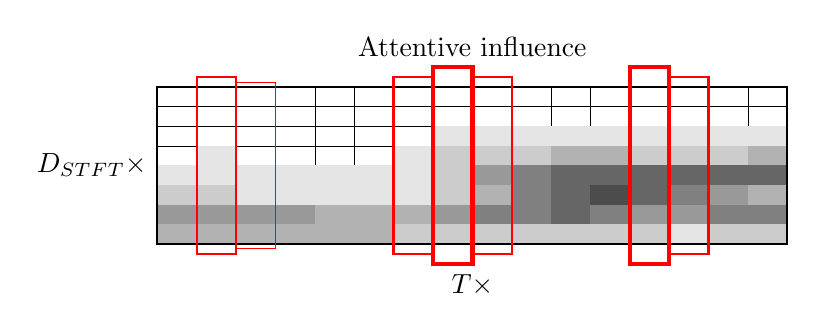
\begin{tikzpicture}[
    very thick,
    arrow/.style={
        -latex,
        very thick,
        rounded corners=0.2cm
    },
    ]

% ------ Grid ------

\draw[transform canvas={xscale=2}, step=0.25cm, ultra thin] (-2, 1) grid (2, 3);
\node[anchor=south] at (0, 3.25) {Attentive influence};
\node[anchor=east] at (-4, 2) {$D_\text{STFT}\times$};
\node[anchor=north] at (0, 0.75) {$T\times$};

% ------ Values ------

\fill[black!30] (-4.0, 1.0) rectangle (-3.5, 1.25);
\fill[black!30] (-3.5, 1.0) rectangle (-3.0, 1.25);
\fill[black!30] (-3.0, 1.0) rectangle (-2.5, 1.25);
\fill[black!30] (-2.5, 1.0) rectangle (-2.0, 1.25);
\fill[black!30] (-2.0, 1.0) rectangle (-1.5, 1.25);
\fill[black!30] (-1.5, 1.0) rectangle (-1.0, 1.25);
\fill[black!20] (-1.0, 1.0) rectangle (-0.5, 1.25);
\fill[black!20] (-0.5, 1.0) rectangle (0.0, 1.25);
\fill[black!20] (0.0, 1.0) rectangle (0.5, 1.25);
\fill[black!20] (0.5, 1.0) rectangle (1.0, 1.25);
\fill[black!20] (1.0, 1.0) rectangle (1.5, 1.25);
\fill[black!20] (1.5, 1.0) rectangle (2.0, 1.25);
\fill[black!20] (2.0, 1.0) rectangle (2.5, 1.25);
\fill[black!10] (2.5, 1.0) rectangle (3.0, 1.25);
\fill[black!20] (3.0, 1.0) rectangle (3.5, 1.25);
\fill[black!20] (3.5, 1.0) rectangle (4.0, 1.25);
\fill[black!40] (-4.0, 1.25) rectangle (-3.5, 1.5);
\fill[black!40] (-3.5, 1.25) rectangle (-3.0, 1.5);
\fill[black!40] (-3.0, 1.25) rectangle (-2.5, 1.5);
\fill[black!40] (-2.5, 1.25) rectangle (-2.0, 1.5);
\fill[black!30] (-2.0, 1.25) rectangle (-1.5, 1.5);
\fill[black!30] (-1.5, 1.25) rectangle (-1.0, 1.5);
\fill[black!30] (-1.0, 1.25) rectangle (-0.5, 1.5);
\fill[black!40] (-0.5, 1.25) rectangle (0.0, 1.5);
\fill[black!50] (0.0, 1.25) rectangle (0.5, 1.5);
\fill[black!50] (0.5, 1.25) rectangle (1.0, 1.5);
\fill[black!60] (1.0, 1.25) rectangle (1.5, 1.5);
\fill[black!50] (1.5, 1.25) rectangle (2.0, 1.5);
\fill[black!40] (2.0, 1.25) rectangle (2.5, 1.5);
\fill[black!40] (2.5, 1.25) rectangle (3.0, 1.5);
\fill[black!50] (3.0, 1.25) rectangle (3.5, 1.5);
\fill[black!50] (3.5, 1.25) rectangle (4.0, 1.5);
\fill[black!20] (-4.0, 1.5) rectangle (-3.5, 1.75);
\fill[black!20] (-3.5, 1.5) rectangle (-3.0, 1.75);
\fill[black!10] (-3.0, 1.5) rectangle (-2.5, 1.75);
\fill[black!10] (-2.5, 1.5) rectangle (-2.0, 1.75);
\fill[black!10] (-2.0, 1.5) rectangle (-1.5, 1.75);
\fill[black!10] (-1.5, 1.5) rectangle (-1.0, 1.75);
\fill[black!10] (-1.0, 1.5) rectangle (-0.5, 1.75);
\fill[black!20] (-0.5, 1.5) rectangle (0.0, 1.75);
\fill[black!30] (0.0, 1.5) rectangle (0.5, 1.75);
\fill[black!50] (0.5, 1.5) rectangle (1.0, 1.75);
\fill[black!60] (1.0, 1.5) rectangle (1.5, 1.75);
\fill[black!70] (1.5, 1.5) rectangle (2.0, 1.75);
\fill[black!60] (2.0, 1.5) rectangle (2.5, 1.75);
\fill[black!50] (2.5, 1.5) rectangle (3.0, 1.75);
\fill[black!40] (3.0, 1.5) rectangle (3.5, 1.75);
\fill[black!30] (3.5, 1.5) rectangle (4.0, 1.75);
\fill[black!10] (-4.0, 1.75) rectangle (-3.5, 2.0);
\fill[black!10] (-3.5, 1.75) rectangle (-3.0, 2.0);
\fill[black!10] (-3.0, 1.75) rectangle (-2.5, 2.0);
\fill[black!10] (-2.5, 1.75) rectangle (-2.0, 2.0);
\fill[black!10] (-2.0, 1.75) rectangle (-1.5, 2.0);
\fill[black!10] (-1.5, 1.75) rectangle (-1.0, 2.0);
\fill[black!10] (-1.0, 1.75) rectangle (-0.5, 2.0);
\fill[black!20] (-0.5, 1.75) rectangle (0.0, 2.0);
\fill[black!40] (0.0, 1.75) rectangle (0.5, 2.0);
\fill[black!50] (0.5, 1.75) rectangle (1.0, 2.0);
\fill[black!60] (1.0, 1.75) rectangle (1.5, 2.0);
\fill[black!60] (1.5, 1.75) rectangle (2.0, 2.0);
\fill[black!60] (2.0, 1.75) rectangle (2.5, 2.0);
\fill[black!60] (2.5, 1.75) rectangle (3.0, 2.0);
\fill[black!60] (3.0, 1.75) rectangle (3.5, 2.0);
\fill[black!60] (3.5, 1.75) rectangle (4.0, 2.0);
\fill[black!10] (-3.5, 2.0) rectangle (-3.0, 2.25);
\fill[black!10] (-1.0, 2.0) rectangle (-0.5, 2.25);
\fill[black!20] (-0.5, 2.0) rectangle (0.0, 2.25);
\fill[black!20] (0.0, 2.0) rectangle (0.5, 2.25);
\fill[black!20] (0.5, 2.0) rectangle (1.0, 2.25);
\fill[black!30] (1.0, 2.0) rectangle (1.5, 2.25);
\fill[black!30] (1.5, 2.0) rectangle (2.0, 2.25);
\fill[black!20] (2.0, 2.0) rectangle (2.5, 2.25);
\fill[black!20] (2.5, 2.0) rectangle (3.0, 2.25);
\fill[black!20] (3.0, 2.0) rectangle (3.5, 2.25);
\fill[black!30] (3.5, 2.0) rectangle (4.0, 2.25);
\fill[black!10] (-0.5, 2.25) rectangle (0.0, 2.5);
\fill[black!10] (0.0, 2.25) rectangle (0.5, 2.5);
\fill[black!10] (0.5, 2.25) rectangle (1.0, 2.5);
\fill[black!10] (1.0, 2.25) rectangle (1.5, 2.5);
\fill[black!10] (1.5, 2.25) rectangle (2.0, 2.5);
\fill[black!10] (2.0, 2.25) rectangle (2.5, 2.5);
\fill[black!10] (2.5, 2.25) rectangle (3.0, 2.5);
\fill[black!10] (3.0, 2.25) rectangle (3.5, 2.5);
\fill[black!10] (3.5, 2.25) rectangle (4.0, 2.5);

% ------ Outline ------
\draw[thick] (-4, 1) -- (4, 1) -- (4, 3) -- (-4, 3) -- cycle;

% ------ Influence ------

\draw[ultra thick, color=red] (-0.5, 0.75) -- (0, 0.75) -- (0, 3.25) -- (-0.5, 3.25) -- cycle;
\draw[ultra thick, color=red] (2, 0.75) -- (2.5, 0.75) -- (2.5, 3.25) -- (2, 3.25) -- cycle;


\draw[thick, color=red] (2.5, 0.875) -- (3, 0.875) -- (3, 3.125) -- (2.5, 3.125) -- cycle;
%\draw[thick, color=red] (1.5, 0.875) -- (2, 0.875) -- (2, 3.125) -- (1.5, 3.125) -- cycle;
\draw[thick, color=red] (0, 0.875) -- (0.5, 0.875) -- (0.5, 3.125) -- (0, 3.125) -- cycle;
\draw[thick, color=red] (-1, 0.875) -- (-0.5, 0.875) -- (-0.5, 3.125) -- (-1, 3.125) -- cycle;
\draw[thick, color=red] (-3.5, 0.875) -- (-3, 0.875) -- (-3, 3.125) -- (-3.5, 3.125) -- cycle;
%\draw[thick, color=red] (-3, 0.875) -- (-2.5, 0.875) -- (-2.5, 3.125) -- (-3, 3.125) -- cycle;

\draw[thin, color=red] (-3, 0.95) -- (-2.5, 0.95) -- (-2.5, 3.05) -- (-3, 3.05) -- cycle;
%\draw[thin, color=red] (3, 0.95) -- (3.5, 0.95) -- (3.5, 3.05) -- (3, 3.05) -- cycle;
%\draw[thin, color=red] (1, 0.95) -- (1.5, 0.95) -- (1.5, 3.05) -- (1, 3.05) -- cycle;
%\draw[thin, color=red] (-1.5, 0.95) -- (-1, 0.95) -- (-1, 3.05) -- (-1.5, 3.05) -- cycle;


\end{tikzpicture}
    \caption{An example of how attention layers allow for attentive influence from from other timeframes spanning large distances. The background is a spectrogram, and the red boxes represent influence in the middle timeframe. The height of the box help visualize influence strength.}
    \label{CTInfluenceFigure}
\end{figure}


Recently, the attention layers have shown great success in \gls{AMT} and \gls{ADT} tasks, in some cases proving superior to the \gls{RNN}~\cite{gardner2022mt3multitaskmultitrackmusic, chang2024yourmt3+, zehren2024analyzingreducingsynthetictorealtransfer}.

Simply replacing the recurrent layers with transformer blocks could allow our model to reap the reward by increasing its ability to understand sequences, while keeping the previously gotten gains from the convolutional layer. Both inside and outside of \gls{ADT}, combining convolutional layers with transformers has seemed beneficial~\cite{zehren2024analyzingreducingsynthetictorealtransfer, gulati2020conformerconvolutionaugmentedtransformerspeech}.

\subsection{Implementation}

Similar to the \gls{CRNN}, an initial fixed-size convolutional block with $I = 2$ is used, with an increasing number of kernels $C = \{32, 64\}$. Then, we project the resulting latent space into a separate, lower dimensional embedding space with dimension $D_e$, before combining it with a sinusoidal positional encoding. 

Following this, the model contains $L$ standard pre-layer normalization transformer block, as these recently have been shown to be more stable during learning than the post-layer versions~\cite{pmlr-v119-xiong20b}. These transformer blocks contain multi-head self-attention layers with $H$ number of heads. Note that the first layer of the feedforward layer inside these transformer blocks uses the \gls{GELU} activation function due to it being the standard within transformers and for its possible performance improvements over \gls{ReLU}~\cite{devlin-etal-2019-bert, hendrycks2023gaussianerrorlinearunits}. Lastly, the linear layer outputs onset probabilities.

\begin{figure}[H]
    \centering
    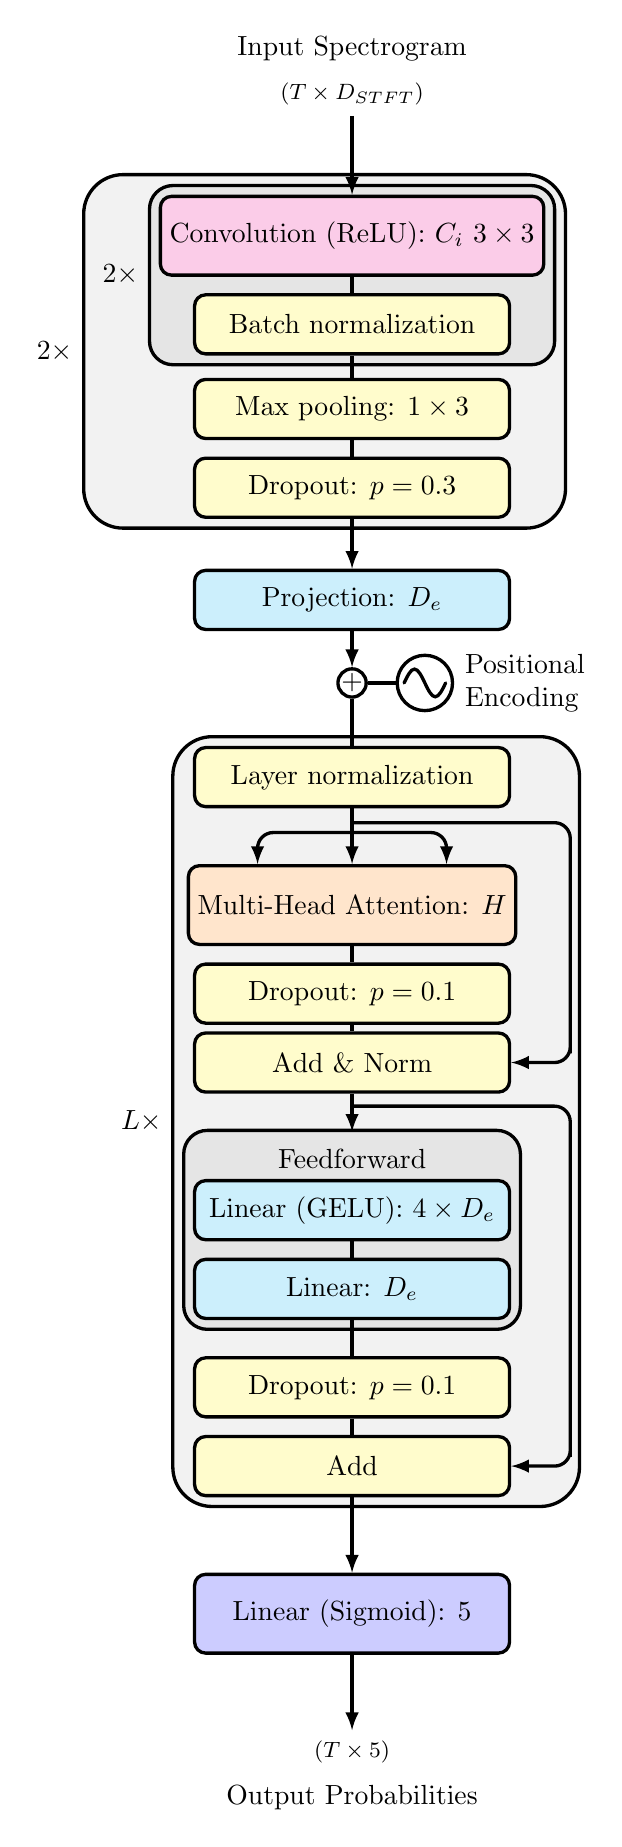
\begin{tikzpicture}[
    very thick,
    arrow/.style={
        -latex,
        very thick,
        rounded corners=0.2cm
    },
    do path picture/.style={%
        path picture={%
          \pgfpointdiff{\pgfpointanchor{path picture bounding box}{south west}}%
            {\pgfpointanchor{path picture bounding box}{north east}}%
          \pgfgetlastxy\x\y%
          \tikzset{x=\x/2,y=\y/2}%
          #1
        }
    },
    sin wave/.style={do path picture={    
        \draw [line cap=round] (-3/4,0)
        sin (-3/8,1/2) cos (0,0) sin (3/8,-1/2) cos (3/4,0);
        }
    }
    ]

\node[anchor=south, label=above:{Input Spectrogram}] at (0, -0.5){\footnotesize{($T \times D_\text{STFT}$)}};

\draw[arrow] (0, -0.5) -- (0, -1.5) node [rectangle,
rounded corners,
draw,
anchor=north,
fill=magenta!20,
minimum height=1cm,
minimum width=4cm
] (a) {Convolution (ReLU): $C_i$  $3 \times 3$};

\draw (a) -- (0, -2.75) node[rectangle,
rounded corners,
draw,
anchor=north,
fill=yellow!20,
minimum height=0.75cm,
minimum width=4cm
] (b) {Batch normalization};

\draw (b) -- (0, -3.825) node[rectangle,
rounded corners,
draw,
anchor=north,
fill=yellow!20,
minimum height=0.75cm,
minimum width=4cm
] (c) {Max pooling: $1 \times 3$};

\draw (c) -- (0, -4.825) node[rectangle,
rounded corners,
draw,
anchor=north,
fill=yellow!20,
minimum height=0.75cm,
minimum width=4cm
] (d) {Dropout: $p = 0.3$};

\begin{scope}[on background layer]
    \node[rectangle,
    fill=gray!20,
    rounded corners=3mm,
    label={[name=ablabel]west:$2\times$},
    draw,
    very thick,
    fit=(a) (b)] (ab) {};
    \node[rectangle,
    fill=gray!10,
    rounded corners=5mm,
    label=west:$2\times$,
    draw,
    very thick,
    fit= (ab) (ablabel) (d)] {};
    \node[rectangle,
    fill=gray!20,
    rounded corners=3mm,
    label={[name=ablabel]west:$2\times$},
    draw,
    very thick,
    fit=(a) (b)] (ab) {};
\end{scope};

\draw[arrow] (d) -- (0, -6.25) node[rectangle,
rounded corners,
draw,
anchor=north,
fill=cyan!20,
minimum height=0.75cm,
minimum width=4cm
] (g) {Projection: $D_e$};

\draw[arrow] (g) -- (0, -7.5) node[circle, 
draw, 
anchor=north,
minimum size=1em, 
inner sep=0pt
] (h) {$\mathbf{+}$};

\node [circle, 
draw, 
sin wave, 
minimum size=2em, 
right=1em of h,
label={[align=left]east:Positional\\Encoding},
] (pe) {};

\draw (pe) -- (h);

\draw (h) -- (0, -8.5) node[rectangle,
rounded corners,
draw,
anchor=north,
fill=yellow!20,
minimum height=0.75cm,
minimum width=4cm
] (i) {Layer normalization};

\draw[arrow] (i) -- (0, -10) node [rectangle,
rounded corners,
draw,
anchor=north,
fill=orange!20,
minimum height=1cm,
minimum width=4cm
] (j) {Multi-Head Attention: $H$};

\draw[arrow] (j.north)++(0, 0.4) -| ($(j.north) + (1.2,0)$);
\draw[arrow] (j.north)++(0, 0.4) -| ($(j.north) + (-1.2,0)$);

\draw (j) -- (0, -11.25) node[rectangle,
rounded corners,
draw,
anchor=north,
fill=yellow!20,
minimum height=0.75cm,
minimum width=4cm
] (k) {Dropout: $p = 0.1$};

\draw (k) -- (0, -12.125) node[rectangle,
rounded corners,
draw,
anchor=north,
fill=yellow!20,
minimum height=0.75cm,
minimum width=4cm
] (l) {Add \& Norm};

\coordinate (larrow) at ($(l.east) + (0.75, 0)$);
\draw[arrow] (j.north)++(0, 0.525) -| (larrow) |- (l.east);

\node[rectangle,
rounded corners,
draw,
anchor=north,
fill=cyan!20,
minimum height=0.75cm,
minimum width=4cm
] at (0, -14) (m) {Linear (GELU): $4 \times D_e$};

\coordinate (m1) at ($(m.north) + (0, 0.5)$);
\draw[arrow] (l) -- ($(m1.north) + (0, 0.1)$);

\draw (m) -- (0, -15) node[rectangle,
rounded corners,
draw,
anchor=north,
fill=cyan!20,
minimum height=0.75cm,
minimum width=4cm
] (n) {Linear: $D_e$};

\draw (n) -- (0, -16.25) node[rectangle,
rounded corners,
draw,
anchor=north,
fill=yellow!20,
minimum height=0.75cm,
minimum width=4cm
] (o) {Dropout: $p = 0.1$};

\draw (o) -- (0, -17.25) node[rectangle,
rounded corners,
draw,
anchor=north,
fill=yellow!20,
minimum height=0.75cm,
minimum width=4cm
] (p) {Add};

\draw[arrow] (m.north)++(0, 0.925) -| ($(p.east) + (0.75, 0)$) |- (p.east);

\begin{scope}[on background layer]

    \node[rectangle,
    fill=gray!20,
    rounded corners=3mm,
    label={[name=mnlabel, yshift=-0.625cm]north:Feedforward},
    draw,
    very thick,
    fit=(m) (m1) (n)] (mn) {};
    \node[rectangle,
    fill=gray!10,
    rounded corners=5mm,
    label=west:$L\times$,
    draw,
    very thick,
    fit= (i) (mn) (p) (larrow)] {};
    \node[rectangle,
    fill=gray!20,
    rounded corners=3mm,
    label={[name=mnlabel, yshift=-0.625cm]north:Feedforward},
    draw,
    very thick,
    fit=(m) (m1) (n)] (mn) {};
\end{scope};

\draw[arrow] (p) -- (0, -19) node[rectangle, 
rounded corners, 
draw, 
anchor=north, 
fill=blue!20,
minimum height=1cm,
minimum width=4cm
] (u) {Linear (Sigmoid): $5$};

\draw[arrow] (u) -- (0, -21);

\node[anchor=north, label=below:{Output Probabilities}] at (0, -21){\footnotesize{($T \times 5$)}};

\end{tikzpicture}
    \caption{Convolutional Transformer architecture structure.}
    \label{CTFigure}
\end{figure}

\begin{table}[H]
    \centering
    \begin{tabular}{lr|c}
        \multicolumn{2}{c|}{Hyperparameter} & Values       \\
        \hline
        $H$ & Number of heads     & \{2, 4, 6, 8\} \\
        $L$ & Number of layers      & \{2, 4, 6, 8, 10\} \\
        $D_e$ & Embedding dimension      & \{72, 144, 288, 576\} \\
    \end{tabular}
    \caption{The different hyperparameters and their respective values tuned to train the Convolutional Transformer.}
    \label{CTHyperparams}
\end{table}

\section{Vision Transformer}

Introducing the Transformer raises a question. Would it be possible for an architecture to be comprised of solely attention layers, removing convolutions and breaking this need for a mixed convolutional-transformer architecture. This question was answered by Google's "An Image Is Worth 16x16 Words"~\cite{dosovitskiy2021imageworth16x16words}, introducing the Vision Transformer.

The Vision Transformer was created to tackle image recognition tasks, though it has been applied to audio classification, displaying great performance on both~\cite{dosovitskiy2021imageworth16x16words, gong2021astaudiospectrogramtransformer}. However, application of the Vision Transformer on an \gls{ADT} task is a novel approach.

It is worth to note that Vision Transformers have been shown to display excellent performance, however they usually need more significantly more data than other architectures to function optimally~\cite{dosovitskiy2021imageworth16x16words}.

\subsection{Patch Embedding}

A key component of the Vision Transformer is the creation of a patch embedding. First, we split the input image into different non-overlapping patches, and flatten them. These patches are linearly projected into a latent space, and a positional encoding is added to retain positional information. This resulting sequence of patches is what is referred to as a patch embedding.

We usually say that patch embeddings eliminate the use of convolutions in the Vision Transformer. However, the actual implementation of splitting the image into patches and linearly projecting each patch are usually implemented with a single 2D convolutional layer. Note that it is a linear projection, meaning the convolutional layer is absent of an activation function.

\begin{figure}[H]
    \centering
    %\input{tikz/patchembedding}
    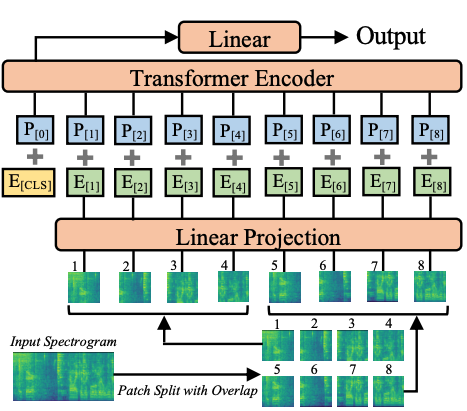
\includegraphics[trim=0 0 0 132, clip, scale=0.7]{figures/patchembedding.png}
    %\textcolor{red}{Insert Patch Embedding visualization.}
    \caption{The creation of a patch embedding from an input spectrogram.}
    \label{PatchEmbeddingFigure}
\end{figure}

\subsection{Architecture Modifications}

Originally, the Vision Transformer has been used on classification tasks where the output is not a sequence. \gls{ADT} is a sequence labeling task, and requires that the output is a sequence, where the time dimension matches the size of the input.

This can be solved by treating a group of patches from the patch embedding together as a timeframe, as long as we ensure that there the number of timeframes are a factor of the number of patches. Then the output of the Vision Transformer could be construed to match our intended output sequence.

\subsection{Implementation}

Initally, we transform the input spectrogram into a ($T \times D_e$) patch embedding. The Convolutional layer splits the spectrogram into ($T \times D_e / P \times P$) different patches. Added to these are a ($D_e / P \times P$) learnable positional embedding, providing positional information to each patch. These are then permuted and flattened, transforming them into our final patch embedding.

Afterwards, we combine it with a sinusoidal positional encoding, and successively apply $L$ transformer blocks with number of heads $H$, identical in structure with those used in the Convolutional Transformer. Lastly, the linear layer outputs onset probabilities.

\begin{figure}[H]
    \hspace*{-0.5cm}
    \centering
    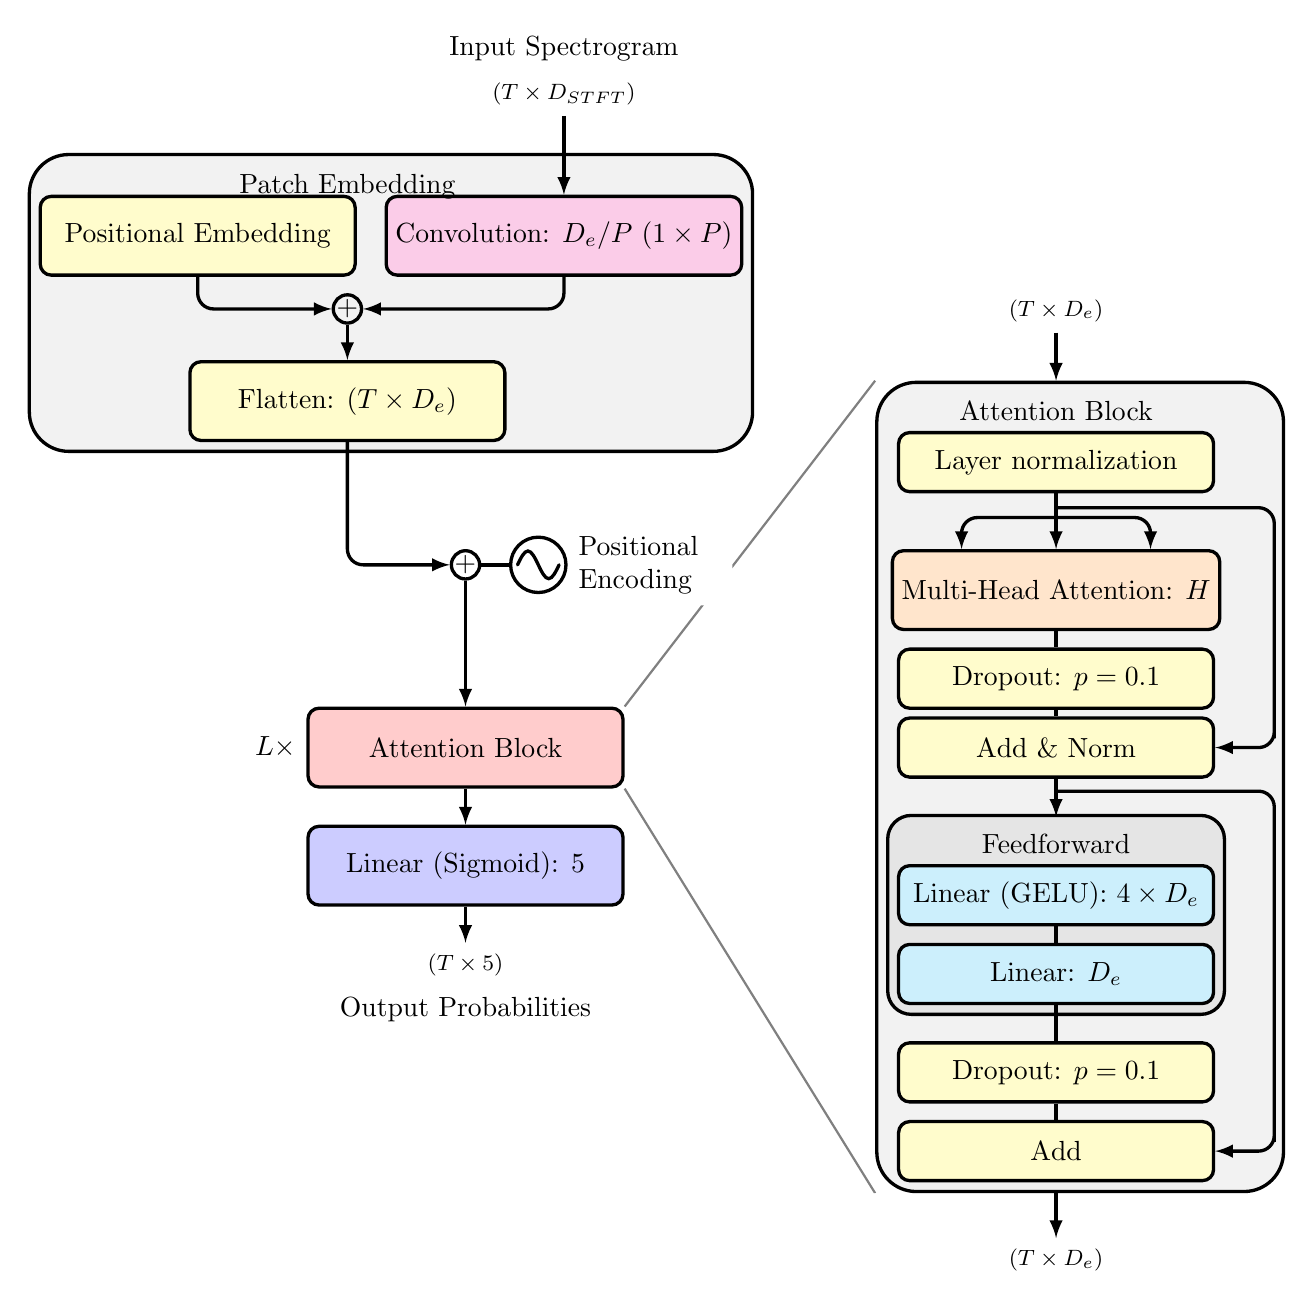
\begin{tikzpicture}[
    very thick,
    arrow/.style={
        -latex,
        very thick,
        rounded corners=0.2cm
    },
    do path picture/.style={%
        path picture={%
          \pgfpointdiff{\pgfpointanchor{path picture bounding box}{south west}}%
            {\pgfpointanchor{path picture bounding box}{north east}}%
          \pgfgetlastxy\x\y%
          \tikzset{x=\x/2,y=\y/2}%
          #1
        }
    },
    sin wave/.style={do path picture={    
        \draw [line cap=round] (-3/4,0)
        sin (-3/8,1/2) cos (0,0) sin (3/8,-1/2) cos (3/4,0);
        }
    }
    ]

\node[anchor=south, label=above:{Input Spectrogram}] at (1.25, -0.5){\footnotesize{($T \times D_\text{STFT}$)}};

\draw[arrow] (1.25, -0.5) -- (1.25, -1.5) node [rectangle,
rounded corners,
draw,
anchor=north,
fill=magenta!20,
minimum height=1cm,
minimum width=4cm
] (a) {Convolution: $D_e/P$ $(1 \times P)$};

\node [rectangle,
rounded corners,
draw,
anchor=north,
fill=yellow!20,
minimum height=1cm,
minimum width=4cm,
left = 1em of a,
] (b) {Positional Embedding};

\node[circle, 
draw, 
anchor=north,
minimum size=1em, 
inner sep=0pt
] at (-1.5, -2.75) (c) {$\mathbf{+}$};

\draw[arrow] (b) |- (c.west);
\draw[arrow] (a) |- (c.east);

\draw [arrow] (c) -- (-1.5, -3.6) node [rectangle,
rounded corners,
draw,
anchor=north,
fill=yellow!20,
minimum height=1cm,
minimum width=4cm,
] (d) {Flatten: $(T \times D_e)$};

\node [anchor=north,
above = 3em of c,
] (e) {Patch Embedding};

\begin{scope}[on background layer]
    \node[rectangle,
    fill=gray!10,
    rounded corners=5mm,
    draw,
    very thick,
    fit= (a) (b) (d) (e)] {};
\end{scope}

\node[circle, 
draw, 
anchor=north,
minimum size=1em, 
inner sep=0pt
] at (0, -6) (h) {$\mathbf{+}$};

\draw[arrow] (d) |- (h);

\node [circle, 
draw, 
sin wave, 
minimum size=2em, 
right=1em of h,
label={[align=left]east:Positional\\Encoding}
] (pe) {};

\draw (pe) -- (h);

\draw[arrow] (h) -- (0, -8) node[rectangle,
rounded corners,
draw,
anchor=north,
minimum size=1em,
inner sep=0pt,
fill=red!20,
minimum height=1cm,
minimum width=4cm,
label={west:$L\times$}
] (v) {Attention Block};

\draw[arrow] (v) -- (0, -9.5) node[rectangle, 
rounded corners, 
draw, 
anchor=north, 
fill=blue!20,
minimum height=1cm,
minimum width=4cm
] (w) {Linear (Sigmoid): $5$};

\draw[arrow] (w) -- (0, -11.0);

\node[anchor=north, label=below:{Output Probabilities}] at (0, -11.0){\footnotesize{($T \times 5$)}};


% ---- Attention Block ----
\draw (7.5, -4.5) node[rectangle,
rounded corners,
draw,
anchor=north,
fill=yellow!20,
label=north:Attention Block,
minimum height=0.75cm,
minimum width=4cm
] (i) {Layer normalization};

\draw[arrow] (i) -- (7.5, -6) node [rectangle,
rounded corners,
draw,
anchor=north,
fill=orange!20,
minimum height=1cm,
minimum width=4cm
] (j) {Multi-Head Attention: $H$};

\draw[arrow] (j.north)++(0, 0.4) -| ($(j.north) + (1.2,0)$);
\draw[arrow] (j.north)++(0, 0.4) -| ($(j.north) + (-1.2,0)$);

\draw (j) -- (7.5, -7.25) node[rectangle,
rounded corners,
draw,
anchor=north,
fill=yellow!20,
minimum height=0.75cm,
minimum width=4cm
] (k) {Dropout: $p = 0.1$};

\draw (k) -- (7.5, -8.125) node[rectangle,
rounded corners,
draw,
anchor=north,
fill=yellow!20,
minimum height=0.75cm,
minimum width=4cm
] (l) {Add \& Norm};

\coordinate (larrow) at ($(l.east) + (0.75, 0)$);
\draw[arrow] (j.north)++(0, 0.525) -| (larrow) |- (l.east);

\node[rectangle,
rounded corners,
draw,
anchor=north,
fill=cyan!20,
minimum height=0.75cm,
minimum width=4cm
] at (7.5, -10) (m) {Linear (GELU): $4 \times D_e$};

\coordinate (m1) at ($(m.north) + (0, 0.5)$);
\draw[arrow] (l) -- ($(m1.north) + (0, 0.1)$);

\draw (m) -- (7.5, -11) node[rectangle,
rounded corners,
draw,
anchor=north,
fill=cyan!20,
minimum height=0.75cm,
minimum width=4cm
] (n) {Linear: $D_e$};

\draw (n) -- (7.5, -12.25) node[rectangle,
rounded corners,
draw,
anchor=north,
fill=yellow!20,
minimum height=0.75cm,
minimum width=4cm
] (o) {Dropout: $p = 0.1$};

\draw (o) -- (7.5, -13.25) node[rectangle,
rounded corners,
draw,
anchor=north,
fill=yellow!20,
minimum height=0.75cm,
minimum width=4cm
] (p) {Add};

\draw[arrow] (m.north)++(0, 0.925) -| ($(p.east) + (0.75, 0)$) |- (p.east);

\coordinate (i1) at ($(i.north) + (0, 0.5)$);

\begin{scope}[on background layer]

    \node[rectangle,
    fill=gray!20,
    rounded corners=3mm,
    label={[name=mnlabel, yshift=-0.625cm]north:Feedforward},
    draw,
    very thick,
    fit=(m) (m1) (n)] (mn) {};
    \node[rectangle,
    fill=gray!10,
    rounded corners=5mm,
    draw,
    very thick,
    fit= (i1) (mn) (p) (larrow)] (imnp) {};
    \node[rectangle,
    fill=gray!20,
    rounded corners=3mm,
    label={[name=mnlabel, yshift=-0.625cm]north:Feedforward},
    draw,
    very thick,
    fit=(m) (m1) (n)] (mn) {};

    \begin{scope}[even odd rule]
        \path[clip] 
        (current bounding box.south west) rectangle (current bounding box.north east)
        ($(pe.north east) + (0, 0.25)$) rectangle ($(pe.south east) + (2.2, -0.25)$);
        \draw[thick, color=black!50] (v.north east) -- (imnp.north west);
        \draw[thick, color=black!50] (v.south east) -- (imnp.south west);
      \end{scope}
\end{scope};

\draw[arrow] (7.5, -3.25) node[anchor=south] {\footnotesize{($T \times D_e$)}} -- (i |- imnp.north);
\draw[arrow] (p |- imnp.south) -- (7.5, -14.75) node[anchor=north] {\footnotesize{($T \times D_e$)}};

\end{tikzpicture}
    \caption{Vision Transformer architecture structure.}
    \label{ViTFigure}
\end{figure}

\begin{table}[H]
    \centering
    \begin{tabular}{lr|c}
        \multicolumn{2}{c|}{Hyperparameter} & Values       \\
        \hline
        $P$ & Patch height      & \{7, 14, 21\} \\
        $H$ & Number of heads     & \{2, 4, 6, 8\} \\
        $L$ & Number of layers      & \{2, 4, 6, 8, 10\} \\
        $D_e$ & Embedding dimension      & \{72, 144, 288, 576\} \\
    \end{tabular}
    \caption{The different hyperparameters and their respective values tuned to train the Vision Transformer.}
    \label{ViTHyperparams}
\end{table}